\documentclass[ucs,9pt]{beamer}

% Copyright 2004 by Till Tantau <tantau@users.sourceforge.net>.
%
% In principle, this file can be redistributed and/or modified under
% the terms of the GNU Public License, version 2.
%
% However, this file is supposed to be a template to be modified
% for your own needs. For this reason, if you use this file as a
% template and not specifically distribute it as part of a another
% package/program, I grant the extra permission to freely copy and
% modify this file as you see fit and even to delete this copyright
% notice.
%
% Modified by Tobias G. Pfeiffer <tobias.pfeiffer@math.fu-berlin.de>
% to show usage of some features specific to the FU Berlin template.

% remove this line and the "ucs" option to the documentclass when your editor is not utf8-capable
\usepackage[utf8x]{inputenc}    % to make utf-8 input possible
\usepackage[ngerman]{babel}     % hyphenation etc., alternatively use 'german' as parameter
\usepackage{amssymb} % Paket für mathematische Formeln
\usepackage{amsmath}
\usepackage{graphicx}
\usepackage[font=scriptsize]{caption}
\usepackage{booktabs} % wissenschaftliche Tabellensätze
\usepackage{makecell}
\usepackage{subcaption}

\usepackage{tikz} % tikz package zum Erstellen von Vektorgraphiken
\usetikzlibrary{shapes.arrows,decorations.pathreplacing}

\include{fu-beamer-template}  % THIS is the line that includes the FU template!
\setbeamertemplate{navigation symbols}{}
\setbeamertemplate{caption}[numbered]

\usepackage{arev,t1enc} % looks nicer than the standard sans-serif font
% if you experience problems, comment out the line above and change
% the documentclass option "9pt" to "10pt"

% image to be shown on the title page (without file extension, should be pdf or png)
\titleimage{ask16_fub.jpg}

\title % [Short Title] (optional, use only with long paper titles)
{Kalibrierung eines Turbulenzmesssystems an einem Motorsegler}

\subtitle{Mastervortrag}

\author[Alexander Bütow] %[Author, Another] % (optional, use only with lots of authors)
{Alexander Bütow}
% - Give the names in the same order as the appear in the paper.

\institute[FU Berlin] % (optional, but mostly needed)
{Institut für Meteorologie, FU Berlin}
% - Keep it simple, no one is interested in your street address.

\date[6.11.2018] % (optional, should be abbreviation of conference name)
{Erstgutachter: Prof. Dr. Jürgen Fischer \\ Zweitgutachter: PD Dr. Peter Névir \\ Betreuer: Dr. Thomas Ruhtz\\[1em] 06.11.2018}
% - Either use conference name or its abbreviation.
% - Not really informative to the audience, more for people (including
%   yourself) who are reading the slides online

\subject{Master Presentation A.Buetow}
% This is only inserted into the PDF information catalog. Can be left
% out.

% you can redefine the text shown in the footline. use a combination of
% \insertshortauthor, \insertshortinstitute, \insertshorttitle, \insertshortdate, ...
\renewcommand{\footlinetext}{\insertshortinstitute, \insertshorttitle, \insertshortdate}
\usepackage[figurename=Abb.,labelfont=scriptsize]{caption}

% Delete this, if you do not want the table of contents to pop up at
% the beginning of each subsection:
\AtBeginSubsection[]
{
  \begin{frame}<beamer>{Inhaltsverzeichnis}
    \tableofcontents[currentsection,currentsubsection]
  \end{frame}
}

\DeclareMathOperator*{\argmax}{arg\,max}

\begin{document}

\begin{frame}[plain]
  \titlepage
\end{frame}

\begin{frame}{Inhaltsverzeichnis}
  \tableofcontents
  % You might wish to add the option [pausesections]
\end{frame}

\section{Einleitung und Motivation}

\begin{frame}{Einleitung und Motivation}
	\begin{itemize}
		\item<1-> Verständnis von Austauschprozessen klimarelevanter Gase in Ökosystemen
		\item<2-> Gasflussmessungen möglich durch \alert{Profiling} (Fluss-Gradient-Ähnlichkeit) und \alert{Eddy-Kovarianzmethode}
		\item<3-> Gastransport eng verknüpft mit turbulenten Vertikalbewegungen:
	\end{itemize}
	\uncover<3->{\begin{equation}
		\overline{F_{k}^{e}}=\rho\overline{w'e'.}\label{eq:turbulenteFlussdichte einer Eigenschaft}
	\end{equation}}
	\uncover<4->{\begin{figure}
		\includegraphics[width=.4\textwidth]{./docmedia/Turbulenzspektrum_original.png}
		\caption{Spektrale Energiedichte, nach Foken (2016) sowie Roedel und Wagner (2011)}
	\end{figure}}
	\begin{itemize}
		\item<5-> \alert{enorme Skalenunterschiede turbulenten Skalentransports}
	\end{itemize}
\end{frame}

\begin{frame}{Einleitung und Motivation}
	\begin{figure}
		\begin{minipage}{0.45\textwidth}
			\includegraphics[width=\textwidth]{./docmedia/cessna.jpg}
			\caption{Cessna T207A Turbo Stationair 8, \textit{D-EAFU}}
		\end{minipage}
		\begin{minipage}{0.45\textwidth}
			\includegraphics[width=\textwidth]{./docmedia/ask16.jpg}
			\caption{Schleicher ASK 16, \textit{D-KMET}}
		\end{minipage}
	\end{figure}
\end{frame}

\begin{frame}{Einleitung und Motivation}
	\addtocounter{figure}{-2}
	\addtocounter{framenumber}{-1}
	\begin{figure}
		\begin{minipage}{0.45\textwidth}
			\includegraphics[width=\textwidth]{./docmedia/cessna_grey.jpg}
			\caption{Cessna T207A Turbo Stationair 8, \textit{D-EAFU}}
		\end{minipage}
		\begin{minipage}{0.45\textwidth}
			\includegraphics[width=\textwidth]{./docmedia/ask16.jpg}
			\caption{Schleicher ASK 16, \textit{D-KMET}}
		\end{minipage}
	\end{figure}
\end{frame}

\section{Grundlagen}

\subsection{Bestimmung des 3D-Windes}

\begin{frame}{Bestimmung des 3D-Windes}
	\begin{itemize}
		\item Transformierung des \textcolor{blue}{relativen Windes am Flugzeug} in \textbf{Erdkoordinaten}
		\item Windvektorbeziehung (\textbf{Erdkoordinaten}):
	\end{itemize}
	
	\begin{align}
		\mathbf{v} = \mathbf{v_p} + \mathbf{v_a} \\
		\mathbf{v_a} = \mathbf{M_t} \textcolor{blue}{\mathbf{v'a}} \\
	\end{align}
	\begin{itemize}
		\item Euler'sche Transformationsmatrix:
	\end{itemize}
	\begin{equation}\small
		\mathbf{M_t} = \left[\begin{array}{ccc}
		cos\Psi cos\Theta & -sin\Psi cos\Phi + cos\Psi sin\Theta sin\Phi & sin\Psi sin\Theta + cos\Psi sin\Theta cos\Phi \\
		sin\Psi cos\Theta & cos\Psi cos\Phi + sin\Psi sin\Theta sin\Phi & sin\Psi sin\Theta cos\Phi - cos\Psi sin\Phi \\
		-sin\Theta & cos\Theta sin\Phi & cos\Theta cos\Phi
		\end{array}\right]
	\end{equation}
\end{frame}

\begin{frame}{Bestimmung des 3D-Windes}
	\begin{figure}
		\small
		\begin{flushleft}
			\begin{minipage}[htbp!]{0.48\textwidth}
				\begin{tikzpicture}[scale=.6, baseline=(current bounding box.north)]
				\draw[->] (0,0) -- (0,4) node[above] {$y$};
				\node[left] at (0,4) {Norden};
				\draw[->] (0,0) -- (4,0) node[right] {$x$};
				\node[above] at (4,0) {Osten};
				\draw[->, dashed, rotate=-30,blue] (0,0) -- (0,3) node[right,blue] {$x'$};
				\draw[->, dashed, rotate=-30,blue] (0,0) -- (3,0) node[right,blue] {$y'$};
				\draw[->, densely dotted, rotate=-45, red] (0,0) -- (0,3);
				\draw[->] (0,2) arc (90:60:2) node[pos=0.5, anchor=north] {$\Psi$};
				\draw[->, rotate=-30, blue]  (0,1.5) arc (90:75:1.5) node[pos=0.1, anchor=north, blue] {$\beta$};
				\node[rotate=-30] (ask16) at (-1,0) {\includegraphics[scale=0.2]{./docmedia/ask16_drauf.png}};
				\end{tikzpicture}
			\end{minipage}
			\begin{minipage}[htbp!]{0.48\textwidth}
				\begin{tikzpicture}[scale=.6, baseline=(current bounding box.north)]
				\draw[->] (0,0) -- (0,4) node[above] {$z$};
				\node[left] at (0,4) {Oben};
				\draw[->] (0,0) -- (4,0) node[right] {$x$};
				\node[above] at (4,0) {Osten};
				\draw[->, dashed, rotate=30, blue] (0,0) -- (3,0) node[right, blue] {$x'$};
				\draw[->, dashed, rotate=120, blue] (0,0) -- (-3,0) node[right, blue] {$z'$};
				\draw[->, densely dotted, rotate=15, red] (0,0) -- (3,0);
				\draw[->] (2,0) arc (0:30:2) node[pos=0.2, left] {$\Theta$};
				\draw[->, rotate=15, blue] (1.5,0) arc (0:15:1.5) node[pos=0.2,left,blue] {$\alpha$};
				\node[rotate=30] (ask16) at (-0.5,-0.1) {\includegraphics[scale=0.2]{./docmedia/ask16_seite_r.png}};
				\draw[->] (2,4) -- (3,4) node[right] {Erd-KO};
				\draw[->, dashed, blue] (2,3.5) -- (3,3.5) node[right, blue] {Flugz.-KO};
				\draw[->, dotted, red] (2,3) -- (3,3) node[right, red] {Track};
				\end{tikzpicture}
			\end{minipage}
			\begin{minipage}{0.6\textwidth}
				\begin{tikzpicture}[scale=.9, baseline=(current bounding box.north)]
				\draw[->] (0,0) -- (0,1) node[above] {$z$};
				\node[above] at (0,1.5) {Oben};
				\draw[->] (3,0) -- (-3,0) node[left] {$y$};
				\node[above] at (-3,0) {Norden};
				\draw[->, dashed, rotate=-30, blue] (0,0) -- (-2,0) node[above, blue] {$y'$};
				\draw[->, dashed, rotate=60, blue] (0,0) -- (-1,0) node[above, blue] {$z'$};
				\draw[->] (-1,0) arc (0:-30:-1) node[pos=0.3, right] {$\Phi$};
				\node[rotate=-30] (ask16) at (0.85,-0.2) {\includegraphics[scale=0.3]{./docmedia/ask16_vorn.png}};
				\end{tikzpicture}
				\label{fig:ko_system}
			\end{minipage}
			\begin{minipage}{0.38\textwidth}
				\caption{Koordinatensysteme}
			\end{minipage}
		\end{flushleft}
	\end{figure}
\end{frame}

\begin{frame}{Bestimmung des 3D-Windes}
	\begin{itemize}
		\item<1-> Messung Raumwinkel: \textbf{Inertial Measuring Unit / Inertial Navigation System (IMU/INS)}
		\item<2-> Anströmwinkel: \textbf{5-Loch-Sonde (5HP)}
	\end{itemize}
	\begin{columns}
		\begin{column}{.4\textwidth}
			\uncover<1->{\begin{figure}
				\includegraphics[width=\textwidth]{./docmedia/igm.png}
				\caption{Novatel SPAN-IGM-A1}
			\end{figure}}
		\end{column}
		\begin{column}{.4\textwidth}
			\uncover<2->{\begin{figure}
				\includegraphics[width=\textwidth]{./docmedia/sonde.jpg}
				\caption{Rosemount 858AJ 5-Loch-Sonde}
			\end{figure}}
		\end{column}
	\end{columns}
\end{frame}

\begin{frame}{Bestimmung des 3D-Windes}
	\begin{figure}
		\begin{minipage}[t]{0.7\textwidth}
			
			\begin{tikzpicture}[scale=0.05]
			\tikzstyle{every node}=[font=\scriptsize]
			
			%Oeffnungen an Probespitze zuerst plotten
			\draw[rotate=10, fill=black] (8.98,8.98) circle (1) node(alp1){} (12.7,0) circle (1) node(p0){} (8.98,-8.98) circle (1) node(alp2){} (8.98,-8.98) ellipse (0.71 and 1) node(bet2){};
			%Statikports
			\draw[rotate=10, fill=black] (-76,0) circle(1) (-76,8.98) ellipse(1 and 0.71) (-76,-8.98) ellipse(1 and 0.71) (-76,12.7) circle (1) (-76,-12.7) circle (1);
			
			%Oeffnungen maskieren
			\draw[white, fill=white, rotate=10] (0,-12.7) arc(90:270:-12.7) -- (0,14) arc(270:90:-14) -- cycle;
			\draw[white, fill=white, rotate=10] (-78,12.7) -- (-74,12.7) -- (-74,14) -- (-78,14);
			\draw[white, fill=white, rotate=10] (-78,-12.7) -- (-74,-12.7) -- (-74,-14) -- (-78,-14);
			
			\draw[->, red] (25,0) -- (-100,0) node[left] {Strömung};
			
			\draw[rotate=10] (-114.3,12.7) -- (0,12.7) arc (270:90:-12.7) -- (-114.3,-12.7); %Probe
			\draw[rotate=10, fill=black] (8.98,0) ellipse (0.71 and 1);
			\draw[rotate=10] (0,0) -- (25,0);
			\draw[rotate=10+45] (0,0) -- (25,0);
			
			\draw[->, rotate=10] (20,0) arc (0:45:20) node[right]{$\tau = 45^\circ$}; %Lochwinkel
			\draw[->, rotate=10, blue] (-40,0) arc (0:-10:-40) node[below left]{$\alpha$}; % Winkel Alpha
			\draw[dashed, rotate=10, blue] (-114.3,0) -- (40,0) node[right] {$x'$}; %x'-Achse
			\draw[densely dotted, rotate=10] (-80,-15) -- (-72,-15) -- (-72,15) -- (-80,15) node[above] {Statikports ($p_{s}$)} -- cycle;
			
			%Beschriftungspfeile
			\draw[->] (30,-15) node[right](x){$p_{\alpha2}$} .. controls +(left:10) .. (alp2);
			\draw[->] (30,10) node[right](x){$p_{\alpha1}$} .. controls +(left:10) .. (alp1);
			\draw[->] (30,2) node[right](x){$p_{0}$} .. controls +(left:10) and +(right:10) .. (p0);
			\end{tikzpicture}
		\end{minipage}
		\hfill
		\begin{minipage}[t]{0.5\textwidth}
			\centering
			\begin{tikzpicture}[scale=0.05]
			\tikzstyle{every node}=[font=\scriptsize]
			
			%Löcher plotten
			\draw (0,0) circle (12.7);
			\draw[fill=black] (0,0) node (p0){} circle (1)
			(0,-8.98) node (alp2){} ellipse (1 and 0.71)
			(0,8.98) node (alp1){} ellipse (1 and 0.71)
			(-8.98,0) node (beta2){} ellipse (0.71 and 1)
			(8.98,0) node (beta1){} ellipse (0.71 and 1);
			
			%Pfeile
			\draw[->] (20,-12) node[right](x){$p_{\alpha2}$} .. controls +(left:10) .. (alp2);
			\draw[->] (20,12) node[right](x){$p_{\alpha1}$} .. controls +(left:10) .. (alp1);
			\draw[->] (20,5) node[right](x){$p_{0}$} .. controls +(left:10) .. (p0);
			\draw[->] (-20,-12) node[left](x){$p_{\beta1}$} .. controls +(right:10) .. (beta1);
			\draw[->] (-20,12) node[left](x){$p_{\beta2}$} .. controls +(right:10) .. (beta2);
			
			\end{tikzpicture}
		\end{minipage}
		\caption{Seiten- (oben) und Vorderansicht (rechts) der 5HP}
		\label{fig:probe_scheme}
	\end{figure}
\end{frame}

\begin{frame}{Bestimmung des 3D-Windes}
	\begin{itemize}
		\item<1-> Erweiterung der Windformel:
	\end{itemize}
	\uncover<1->{\begin{equation}
		\mathbf{v} = \mathbf{v_p} + \mathbf{M_t \textcolor{blue}{v_a'}}
	\end{equation}}
	\uncover<2->{\begin{equation}
		\textcolor{blue}{\mathbf{v_a'} = -\textcolor{red}{v_m} D^{-1}\left(\begin{array}{c}
		1 \\ tan \beta \\ tan \alpha
		\end{array}\right)}
	\end{equation}}
	\uncover<2->{\begin{equation}
		\textcolor{blue}{D=\frac{1}{\sqrt{1 + tan^2 \alpha + tan^2 \beta}}}
	\end{equation}}
	\uncover<3->{\begin{equation}
		\mathbf{v} = \mathbf{v_p} + \mathbf{M_t}\mathbf{\textcolor{blue}{v_a'}} + \boldsymbol{\omega} \times \mathbf{M_t}\mathbf{\textcolor{blue}{l'}}
	\end{equation}}
	\begin{itemize}
		\item<4-> Vereinfachung: $\textcolor{blue}{\mathbf{l'}=\left(\begin{array}{c}
			l \\ 0 \\ 0
			\end{array}\right)}$
	\end{itemize}
\end{frame}

\begin{frame}{Bestimmung des 3D-Windes}
	\begin{itemize}
		\item vollständiger Formelsatz:
	\end{itemize}
	\begin{equation}
		\begin{split}
			u=\textcolor{blue}{-}\textcolor{red}{v_m}\textcolor{blue}{D^{-1}}[\sin\Psi\cos\Theta + \textcolor{blue}{\tan\beta}(\cos\Psi\cos\Phi + \sin\Psi\sin\Theta\sin\Phi) \\
			+ \textcolor{blue}{\tan\alpha}(\sin\Psi\sin\Theta\cos\Phi - \cos\Psi\sin\Phi)] \\
			+  v_{x} - \textcolor{blue}{l}(\dot{\Theta}\sin\Theta\sin\Psi - \dot{\Psi}\cos\Psi\cos\Theta)\\ 
			\\
			v=\textcolor{blue}{-}\textcolor{red}{v_m}\textcolor{blue}{D^{-1}}[\cos\Psi\cos\Theta - \textcolor{blue}{\tan\beta}(\sin\Psi\cos\Phi - \cos\Psi\sin\Theta\sin\Phi) \\
			+ \textcolor{blue}{\tan\alpha}(\cos\Psi\sin\Theta\cos\Phi + \sin\Psi\sin\Phi)] \\
			+ v_{y} - \textcolor{blue}{l}(\dot{\Psi}\sin\Psi\cos\Theta + \dot{\Theta}\cos\Psi\sin\Theta) \\ 
			\\
			w=\textcolor{blue}{-}\textcolor{red}{v_m}\textcolor{blue}{D^{-1}}(\sin\Theta - \textcolor{blue}{\tan\beta}\cos\Theta\sin\Phi - \textcolor{blue}{\tan\alpha}\cos\Theta\cos\Phi) \\
			+ v_{w} + \textcolor{blue}{l}\dot{\Theta}\cos\Theta
		\end{split}
	\end{equation}
\end{frame}

\subsection{Wahre Fluggeschwindigkeit (TAS)}

\begin{frame}{Wahre Fluggeschwindigkeit (TAS)}
	\begin{itemize}
		\item<1-> Bestimmung der True Airspeed (TAS) bzw. $\textcolor{red}{v_m}$
		\item<2-> Energieerhaltung nach Bernoulli (vereinfacht):
	\end{itemize}
	\uncover<2->{\begin{equation}\small
		\frac{u_1^2}{2}+c_{p}T_{1}=\frac{u_2^2}{2}+c_{p}T_{2} = const.
	\end{equation}}
	\begin{itemize}
		\item<3-> im Staupunkt: $u_2=0, u_1=\textcolor{red}{v_m}, T_2=T_0$
		\begin{itemize}
			\item $T_0$: totale Temperatur (TAT), $T_s$: (hydro-)statische Temperatur
		\end{itemize}
	\end{itemize}
	\uncover<3->{\begin{equation}
		v_m^2 = 2c_p(T_0-T_s)
	\end{equation}}
	\begin{itemize}
		\item<4-> potentielle Temperatur (Aerodynamik: Isentropenbeziehung):
	\end{itemize}
	\uncover<4->{\begin{align}\small
		T_s = T_0\left(\frac{p_s}{p_0}\right)^{\frac{\kappa - 1}{\kappa}} \\
		q = p_0 - p_s
	\end{align}
	\begin{equation}\small
		v_m^2 = 2 c_p T_s \left[\left(\frac{p_0}{p_s}\right)^{\frac{\kappa - 1}{\kappa}} - 1\right]
	\end{equation}}
	\begin{itemize}
		\item<5-> Alternative Darstellung mit der Mach-Zahl:
	\end{itemize}
	\uncover<5->{\begin{equation}\small
		v_m^2 = \kappa R T_s M^2
	\end{equation}}
\end{frame}

\begin{frame}{Wahre Fluggeschwindigkeit (TAS)}
	\begin{itemize}
		\item<1-> Problem bei Temperaturmessung: kein idealer Aufstau, diabatische Verluste etc.
		\item<2-> Einführung eines Recovery-Factors:
	\end{itemize}
	\begin{columns}
		\begin{column}[t]{0.45\textwidth}
			\uncover<2->{\begin{equation}
				r=\frac{T_r - T_s}{T_0 - T_s}
			\end{equation}}
			\uncover<3->{\begin{equation}
				T_s=\frac{T_r}{r\left(\frac{p_0}{p_s}\right)^{\frac{\kappa - 1}{\kappa}} + (1 - r)}
			\end{equation}}
			\uncover<4->{\begin{equation}
				v_{m}=\sqrt{\frac{\kappa R M^2 T_r}{r\left(\frac{\kappa - 1}{2}\right) M^2 + 1}}
			\end{equation}}
		\end{column}
		\begin{column}[t]{0.5\textwidth}
			\uncover<1->{\begin{figure}
				\centering
				\includegraphics[width=.5\textwidth]{./docmedia/e102.jpg}
				\qquad
				\includegraphics[width=.5\textwidth]{./docmedia/hmt311.jpg}
				\caption{Rosemount 102E TAT-Housing (oben), Vaisala HMT311 (unten)}
			\end{figure}}
		\end{column}
	\end{columns}
\end{frame}

\subsection{Messung der Anströmwinkel}

\begin{frame}{Messung der Anströmwinkel}
	\uncover<1->{\begin{figure}
		\begin{tikzpicture}[scale=0.03]
			\tikzstyle{every node}=[font=\scriptsize]
			
			%Oeffnungen an Probespitze zuerst plotten
			\draw[rotate=10, fill=black] (8.98,8.98) circle (1) node(alp1){} (12.7,0) circle (1) node(p0){} (8.98,-8.98) circle (1) node(alp2){} (8.98,-8.98) ellipse (0.71 and 1) node(bet2){};
			%Statikports
			\draw[rotate=10, fill=black] (-76,0) circle(1) (-76,8.98) ellipse(1 and 0.71) (-76,-8.98) ellipse(1 and 0.71) (-76,12.7) circle (1) (-76,-12.7) circle (1);
			
			%Oeffnungen maskieren
			\draw[white, fill=white, rotate=10] (0,-12.7) arc(90:270:-12.7) -- (0,14) arc(270:90:-14) -- cycle;
			\draw[white, fill=white, rotate=10] (-78,12.7) -- (-74,12.7) -- (-74,14) -- (-78,14);
			\draw[white, fill=white, rotate=10] (-78,-12.7) -- (-74,-12.7) -- (-74,-14) -- (-78,-14);
			
			\draw[->, red] (25,0) -- (-100,0) node[left] {Strömung};
			
			\draw[rotate=10] (-114.3,12.7) -- (0,12.7) arc (270:90:-12.7) -- (-114.3,-12.7); %Probe
			\draw[rotate=10, fill=black] (8.98,0) ellipse (0.71 and 1);
			\draw[rotate=10] (0,0) -- (25,0);
			\draw[rotate=10+45] (0,0) -- (25,0);
			
			\draw[->, rotate=10] (20,0) arc (0:45:20) node[right]{$\tau = 45^\circ$}; %Lochwinkel
			\draw[->, rotate=10, blue] (-40,0) arc (0:-10:-40) node[below left]{$\alpha$}; % Winkel Alpha
			\draw[dashed, rotate=10, blue] (-114.3,0) -- (45,0) node[right] {$x'$}; %x'-Achse
			\draw[densely dotted, rotate=10] (-80,-15) -- (-72,-15) -- (-72,15) -- (-80,15) node[above] {Statikports ($p_{s}$)} -- cycle;
			
			%Beschriftungspfeile
			\draw[->] (30,-15) node[right](x){$p_{\alpha2}$} .. controls +(left:10) .. (alp2);
			\draw[->] (30,10) node[right](x){$p_{\alpha1}$} .. controls +(left:10) .. (alp1);
			\draw[->] (30,2) node[right](x){$p_{0}$} .. controls +(left:10) and +(right:10) .. (p0);
		\end{tikzpicture}
	\end{figure}}
	\begin{itemize}\small
		\item<2-> potentialtheoretische Druckbeiwertverteilung ($c_p$) auf einer Kugeloberfläche:
	\end{itemize}
	\begin{columns}
		\begin{column}[t]{0.65\textwidth}
			\uncover<2->{\begin{equation}\footnotesize
				c_p = \frac{p_x-p_s}{q} = 1-\frac{9}{4}sin^2\theta
			\end{equation}}
			\uncover<3->{\begin{equation}\footnotesize
				c_{p} = 1-\frac{9}{4}sin^2(\alpha \pm \tau)
			\end{equation}}
			\uncover<4->{\begin{equation}\footnotesize
				\frac{p_{\alpha 2}-p_{\alpha 1}}{q} = \Delta \tilde{p_{\alpha}} = \frac{9}{4}\left(sin^2(\alpha +\tau)-sin^2(\alpha -\tau)\right)
			\end{equation}}
			\uncover<5->{\begin{equation}\footnotesize
				\Delta \tilde{p_{\alpha}} = \frac{9}{4}sin(2\alpha)
			\end{equation}}
			\uncover<6->{\begin{equation}\footnotesize
				\alpha = \frac{1}{2}arcsin\left(\frac{4}{9}\Delta \tilde{p_{\alpha}}\right)
			\end{equation}}
			\uncover<7->{\begin{equation}\footnotesize
				\alpha\approx \frac{2}{9}\Delta \tilde{p_{\alpha}}=\frac{1}{C_k} \Delta \tilde{p_{\alpha}}
			\end{equation}}
		\end{column}
		\begin{column}[t]{0.35\textwidth}
			\uncover<8->{\begin{figure}
				\includegraphics[width=0.45\textwidth]{./docmedia/cpt6100.jpg}
				\caption{Drucksensor Mensor CPT6100}
			\end{figure}}
		\end{column}
	\end{columns}
\end{frame}

\section{Aufbau des Messsystems}

\subsection{Geräte}

\begin{frame}{Geräte}
	\begin{columns}
		\begin{column}[t]{0.45\textwidth}
			\begin{figure}
				\includegraphics[width=\textwidth]{./docmedia/ask16.jpg}
				\qquad
				\includegraphics[width=\textwidth]{./docmedia/sonde.jpg}
				\qquad
				\includegraphics[width=.2\textwidth]{./docmedia/cpt6100.jpg}
			\end{figure}
		\end{column}
		\begin{column}[t]{0.45\textwidth}
			\begin{figure}
				\includegraphics[width=0.4\textwidth]{./docmedia/igm.png}
				\qquad
				\includegraphics[width=.4\textwidth]{./docmedia/hmt311.jpg}
				\qquad
				\includegraphics[width=\textwidth]{./docmedia/raspi.jpg}
				\caption{(v.l.o.n.r.u) ASK 16, 5HP, Mensor CPT6100, Novatel SPAN-IGM-A1, Vaisala HMT 311, Raspberry Pi 3 (Quelle: Raspberry Pi Foundation)}
			\end{figure}
		\end{column}
	\end{columns}
\end{frame}

\begin{frame}{Geräte}
	\begin{columns}
		\begin{column}{.45\textwidth}
			\begin{figure}
				\includegraphics[width=\textwidth]{./docmedia/wingpod_oberseite.jpg}
				\qquad
				\includegraphics[width=\textwidth]{./docmedia/wingpod_unterseite.jpg}
			\end{figure}
		\end{column}
		\begin{column}{.45\textwidth}
			\begin{figure}
				\includegraphics[width=\textwidth]{./docmedia/wingpod_whole.jpg}
			\end{figure}
		\end{column}
	\end{columns}
\end{frame}

\begin{frame}{Geräte}
	\begin{figure}
		\includegraphics[width=\textwidth]{./docmedia/scheme.png}
	\end{figure}
\end{frame}

\section{Kalibrierung}

\subsection{Zu lösende Probleme}

\begin{frame}{Zu lösende Probleme}
	\begin{itemize}
		\item<1-> Zu lösende Probleme:
		\begin{itemize}
			\item<2-> Synchronisierung
			\item<3-> Sensorfehler
			\item<4-> Aerodynamische Einflüsse
		\end{itemize}
	\end{itemize}
	\uncover<5->{\begin{figure}
		\includegraphics[width=0.4\textwidth]{./docmedia/airfoil_stream.jpg}
		\qquad
		\includegraphics[width=0.4\textwidth]{./docmedia/halo.jpg}
		\caption{Stromlinien um Profil (links), Nasenmast des Forschungsflugzeugs \textit{HALO} (Quelle: DLR)}
	\end{figure}}
	\begin{itemize}
		\item<6-> \alert{Isolierung der Fehlerquellen}
	\end{itemize}
\end{frame}

\subsection{Synchronisierung}

\begin{frame}{Synchronisierung}
	\begin{itemize}
		\item<1-> Latenz und Jitter:
	\end{itemize}
	\uncover<1->{\begin{equation}
		t_{S,i}=t_{i}+t_{d,i}+\underbrace{t_{res}+t_{kon,i}+t_{kom,i}}_{t_{lat,i}}
	\end{equation}}
	\uncover<2->{\begin{equation}
		\hat{t_{S,i}}=t_{i}+\hat{t_{d,i}}+\overline{t_{lat}}
	\end{equation}}
	\uncover<3->{\begin{table}
		\centering
		\caption{Übersicht der Latenz- und Jitterwerte für alle Sensoren/Logs}
		\scriptsize
		\begin{tabular}{lccccc}
			\toprule
			Gerät & Log & Formelzeichen & \makecell{$t_{int}$ \\ in 10$^{-3}$ s} & \makecell{$\sigma_{jit}$ \\ in 10$^{-3}$ s} & \makecell{$\sigma_{\hat{jit}}$ \\ in 10$^{-3}$ s} \\
			\midrule
			CPT6100 & p\_alp & $\Delta p_\alpha$ & 20.26 & 7.07 & 0.01 \\
			& p\_bet & $\Delta p_{\beta}$ & 20.31 & 7.10 & 0.01 \\
			& p\_alt & $p_s$ & 20.24 & 7.05 & 0.01 \\
			& p\_spd & $q$ & 20.27 & 7.06 & 0.01 \\
			\midrule
			SPAN-IGM-A1 & nova0 & $(t,\dot{\Theta},\dot{\Psi},\ddot{x'},\ddot{y'},\ddot{z'})$ & 50.00 & 4.30 & 0.01 \\
			& nova1 & $(t,$ lat, lon, $h,v_x,v_y,v_z,\Psi,\Theta,\Phi)$ & 50.00 & 6.39 & 0.01 \\
			\midrule
			HMT311 & hmt & $(T,r_F)$ & 535.09 & 9.41 & 1.30 \\
			\midrule
			USB-1608FS-PLUS & usb1608 & $U$ & 20.00 & 0.06 & 0.01 \\
			\bottomrule
		\end{tabular}
	\end{table}}
\end{frame}

\begin{frame}{Synchronisierung}
	\begin{itemize}
		\item<1-> Relative Synchronisierung zwischen Druck- und IMU-Messwerten:
	\end{itemize}
	\uncover<1->{\begin{equation}
		\overline{t_{lat,rel}}=\overline{t_{lat,CPT}}-\overline{t_{lat,IMU}}
	\end{equation}}
	\uncover<2->{\begin{equation}
		\overline{t_{lat,rel}}=\overline{t_{lat,CPT}}
	\end{equation}}
	\begin{itemize}
		\item<3->\alert<3>{Nächster Schritt: Quantifizierung von $\overline{t_{lat,CPT}}$}
		\item<4-> Kreuzkorrelation zwischen IMU- und Druckmesswerten
	\end{itemize}
	\uncover<4->{\begin{equation}\small
		R_{xy}=\frac{Cov(X,Y)}{\sigma_x \sigma_y}=\frac{\frac{1}{n-1} \sum\limits_{i=1}^{n}\left[\left(x_{i}-\overline{x}\right)\left(y_{i}-\overline{y}\right)\right]}{\left[\frac{1}{n-1}\sum\limits_{i=1}^{n}\left(x_{i}-\overline{x}\right)^{2}\right]^{1/2}\left[\frac{1}{n-1}\sum\limits_{i=1}^{n}\left(y_{i}-\overline{y}\right)^{2}\right]^{1/2}}
	\end{equation}}
	\uncover<5->{\begin{equation}\small
		k_{max}=\argmax_{k \in D}\left[\frac{\frac{1}{n-k-1} \sum\limits_{i=1}^{n-k}\left[\left(x_{i}-\overline{x}\right)\left(y_{i+k}-\overline{y}\right)\right]}{\left[\frac{1}{n-k-1}\sum\limits_{i=1}^{n-k}\left(x_{i}-\overline{x}\right)^{2}\right]^{1/2}\left[\frac{1}{n-k-1}\sum\limits_{i=1}^{n-k}\left(y_{i+k}-\overline{y}\right)^{2}\right]^{1/2}}\right]
	\end{equation}}
	\begin{itemize}
		\item<5-> \alert{Latenzzeit: $\tau=t_{int}\cdot k_{max}$}
	\end{itemize}
\end{frame}

\begin{frame}{Synchronisierung}
	\begin{itemize}
		\item<1-> Definition Auftriebskoeffizient:
	\end{itemize}
	\uncover<1->{\begin{equation}
		c_a=\frac{F'}{ql_s}=2\pi(\alpha-\alpha_0)
	\end{equation}}
	\begin{itemize}
		\item<2-> \alert<2>{Anstellwinkel $\alpha$ $\Longleftrightarrow$ Vertikalbeschleunigung entlang $\ddot{z}'$}
		\item<3-> Berücksichtigung der Mastlänge $l$:
	\end{itemize}
	\uncover<3->{\begin{equation}
		t_{l}=\frac{l}{v_m}
	\end{equation}}
	\uncover<4->{\begin{equation}
		\overline{t_{lat,rel}}=\overline{t_{lat,CPT}}-t_l
	\end{equation}}
\end{frame}

\begin{frame}{Synchronisierung}
	\begin{figure}
	 	\includegraphics[width=.8\textwidth]{./docmedia/p_lag_fit.pdf}
	 	\caption{Kreuzkorrelationen zwischen der IMU und Drucksensoren}
	\end{figure}
\end{frame}

\subsection{Sensorfehler}

\begin{frame}{Sensorfehler}
	\begin{itemize}
		\item<1-> IMU: Korrekturen nicht ohne weiteres möglich
		\item<2-> Drucksensoren: Einfluss von Beschleunigungen und Temperatur?
	\end{itemize}
	\uncover<2->{\begin{figure}
		\includegraphics[width=.6\textwidth]{./docmedia/temp_torture_ascent_1.pdf}
		\caption{Versuch in der Klimakammer}
	\end{figure}}
	\begin{itemize}
		\item<3-> Temperatureinfluss signifikant ab $T\approx0^\circ C$
		\item<4-> $\Delta p_{\alpha}=0.1\ mbar \Rightarrow \Delta w = \pm 2.2\cdot 10^{-3} m\ s^{-1} \Rightarrow$ vernachlässigbar
		\item<5-> Korrektur möglich, Applikation technisch aufwendig
	\end{itemize}
\end{frame}

\subsection{Korrektur aerodynamischer Einflüsse}

\begin{frame}{Korrektur aerodynamischer Einflüsse}
	\begin{itemize}
		\item<1-> Einführung heuristischer Korrekturfunktionen
		\item<2-> Korrektur statischer Druckfehler:
	\end{itemize}
	\uncover<2->{\begin{align}
		p_{s,c} = p_{s,i} - \textcolor{red}{C_{s2,q}}q_i^2 - \textcolor{red}{C_{s1,q}}q_i - \textcolor{red}{p_{s,0}} \\
		q_{c} = q_i + \textcolor{red}{C_{s2,q}}q_i^2 + \textcolor{red}{C_{s1,q}}q_i +\textcolor{red}{q_{i,0}}
	\end{align}}
	\begin{itemize}
		\item<3-> Korrektur dynamischer Druckfehler:
	\end{itemize}
	\uncover<3->{\begin{equation}
		q_{c,c} = q_c + \textcolor{red}{C_{q,q}}q_c
	\end{equation}}
	\begin{itemize}
		\item<4-> Korrektur Anströmwinkel:
	\end{itemize}
	\uncover<4->{\begin{align}
		\alpha = \frac{1}{\textcolor{red}{C_{k,\alpha}}}\Delta \tilde{p} - \textcolor{red}{\alpha_0} \\
		\beta = \frac{1}{\textcolor{red}{C_{k,\beta}}}\Delta \tilde{p} - \textcolor{red}{\beta_0}
	\end{align}}
\end{frame}

\begin{frame}{Korrektur aerodynamischer Einflüsse}
	\begin{itemize}
		\item<1-> \alert<1>{Ausführen von Kalibrierungsmanövern}, Minimierung von $\sigma_{u}, \sigma_{v}, \sigma_{w}$
		\item<2-> Manöver zur Kalibrierung des statischen und dynamischen Drucks:
	\end{itemize}
	\uncover<2->{\begin{figure}
		\begin{subfigure}{0.25\textwidth}
			\begin{tikzpicture}[scale=0.5, baseline=(current bounding box.north)]
			\tikzstyle{every node}=[font=\scriptsize]
			\node[rotate=-60] (airplane) at (0,0) {\includegraphics[scale=0.07]{./docmedia/airplane_top.png}};
			\draw[->,thick, rotate=-60] (0,0) -- (0,5);
			\draw[->,thick, rotate=-60] (0,5) arc (0:45:1.6) coordinate (leg);
			\draw[thick,rotate=-60] (leg) arc (45:-180:-0.3) -- (0,5);
			\draw[->,thick, rotate=-60] (0,5) -- (0,1);
			\draw[->,thick, rotate=-60] (0,0) arc (0:45:-1.6) coordinate (leg2);
			\draw[thick,rotate=-60] (leg2) arc (45:-180:0.3) -- (0,0);
			
			\draw[->, >=latex, blue!40, line width=7pt, rotate=-60] (1,3) -- node [black,rotate=30] {Wind} (1,0);
			\draw [decorate,decoration={brace,amplitude=5pt,raise=5pt},yshift=10pt,rotate=-60] (0,0) -- (0,5) node [black,midway,xshift=-10pt,yshift=10pt,rotate=30] {\tiny$\approx 30 - 60$ s};
			\end{tikzpicture}
		\end{subfigure}
		\begin{subfigure}{0.25\textwidth}
			\begin{tikzpicture}[scale=1, baseline=(current bounding box.north)]
			\tikzstyle{every node}=[font=\scriptsize]
			\node (airplane) at (0,0) {\includegraphics[scale=0.07]{./docmedia/airplane_top.png}};
			\draw[->,thick] (airplane) arc (0:60:1) coordinate (pnt1);
			\draw[->,thick] (pnt1) arc(60:240:1) coordinate (pnt2);
			\draw[thick] (pnt2) arc (240:360:1) (airplane);
			\end{tikzpicture}
		\end{subfigure}
		\begin{subfigure}{0.25\textwidth}
			\begin{tikzpicture}[scale=1, baseline=(current bounding box.north)]
			\tikzstyle{every node}=[font=\scriptsize]
			\node (start) at (0,0) {\includegraphics[scale=0.07]{./docmedia/airplane_top.png}};
			\draw[thick] (start) -- (0,2) coordinate (leg1_e);
			\draw[thick] (leg1_e) arc(0:90:0.5) coordinate (leg2_b);	
			\draw[->,thick] (leg2_b) -- (-2.5,2.5) coordinate (leg2_e);
			\draw[thick] (leg2_e) arc(90:180:0.5) coordinate (leg3_a);
			\draw[thick] (leg3_a) -- (-3,0) coordinate (leg3_e);
			\draw[thick] (leg3_e) arc(180:270:0.5) coordinate (leg4_a);
			\draw[->,thick] (leg4_a) -- (-0.5,-0.5) coordinate (leg4_e);
			\draw[thick] (leg4_e) arc(270:360:0.5);
			
			\draw[->, >=latex, blue!40, line width=7pt] (-1.5,2) -- node [black,rotate=90] {Wind} (-1.5,0);
			\draw [decorate,decoration={brace,amplitude=5pt,mirror,raise=5pt},yshift=0pt](-2.5,-0.5) -- (-0.5,-0.5) node [black,midway,yshift=-0.5cm] {\tiny$\approx 30 - 60$ s};
			\end{tikzpicture}
		\end{subfigure}
		\begin{subfigure}{0.25\textwidth}
			\begin{tikzpicture}[scale=1, baseline=(current bounding box.north)]
			\draw[->,thick] (0,0) -- (0.5,0);
			\draw[thick] (0.5,0) -- (1,0);
			\node (pic) at (1,0.05) {\includegraphics[scale=0.07,angle=20]{./docmedia/airplane_side.png}};
			\node[below] at (pic) {\tiny $v_{ias} \gtrsim v_{Stall}$};
			\draw[thick] (1,0) -- (3.5,0);
			\node (pic2) at (3.5,0.05) {\includegraphics[scale=0.07,angle=-5]{./docmedia/airplane_side.png}};
			\node[below] at (pic2) {\tiny $v_{ias} \lesssim v_{NE}$};
			\draw[->,thick] (3.5,0) -- (4,0);
			\end{tikzpicture}
		\end{subfigure}
		\caption{Variation von Kalibriermanövern zur Kalibrierung von $q$ und $p_s$}
	\end{figure}}
\end{frame}

\begin{frame}
	\begin{itemize}
		\item Kalibriermanöver für Anströmwinkel $\alpha$ und $\beta$:
	\end{itemize}
	\begin{figure}
		\begin{tikzpicture}[scale=1, baseline=(current bounding box.north)]
		\draw[->,thick] (0,0) sin(1,.2);
		\draw[->,thick] (1,.2) cos(2,0) sin(3,-.2) cos(4,0) sin(5,.2) cos(6,0) sin(7,-.2) cos(8,0);
		\node (pic) at (2,0) {\includegraphics[scale=0.07,angle=-10]{./docmedia/airplane_side.png}};
		\node (pic2) at (5,.25) {\includegraphics[scale=0.07,angle=5]{./docmedia/airplane_side.png}};
		\draw [decorate,decoration={brace,amplitude=5pt,raise=5pt,mirror},yshift=0pt](1,-0.5) -- (5,-0.5) node [black,midway,yshift=-0.5cm] {\tiny$\approx 5$ s};
		\end{tikzpicture}
		\caption{Pitch-Oszillationen zur Ermittlung von $C_{k,\alpha}$ (Seitenansicht).}
	\end{figure}
	\begin{figure}
		\begin{tikzpicture}[scale=1, baseline=(current bounding box.north)]
		\draw[->,thick] (0,0) -- (1,0);
		\draw[->,thick] (1,0) -- (6,0);
		\node (pic) at (1.5,0) {\includegraphics[scale=0.07,angle=-75]{./docmedia/airplane_top.png}};
		\node (pic2) at (3,0) {\includegraphics[scale=0.07,angle=-105]{./docmedia/airplane_top.png}};
		\node (pic3) at (4.5,0) {\includegraphics[scale=0.07,angle=-75]{./docmedia/airplane_top.png}};
		\draw [decorate,decoration={brace,amplitude=5pt,raise=5pt,mirror},yshift=0pt](1.5,-.3) -- (4.5,-.3) node [black,midway,yshift=-0.5cm] {\tiny$\approx 10$ s};
		\end{tikzpicture}
		\caption{Yaw-Oszillation zur Ermittlung von $C_{k,\beta}$ (Draufsicht).}
	\end{figure}
\end{frame}

\subsection{Flüge}

\begin{frame}{Flüge}
	\begin{itemize}
		\item Ausführung mehrerer Flüge im August 2017 und Juni/Juli 2018
		\item Teilnahme an zweitägiger Messkampagne bei Demmin (Mecklenburg-Vorpommern)
	\end{itemize}
	\begin{columns}
		\begin{column}{0.48\textwidth}
			\begin{figure}
				\includegraphics[width=\textwidth]{./docmedia/demmin_ready.jpg}
				\caption{ASK 15 am Flugplatz Neubrandenburg-Trollenhagen}
			\end{figure}
		\end{column}
		\begin{column}{0.48\textwidth}
			\begin{figure}
				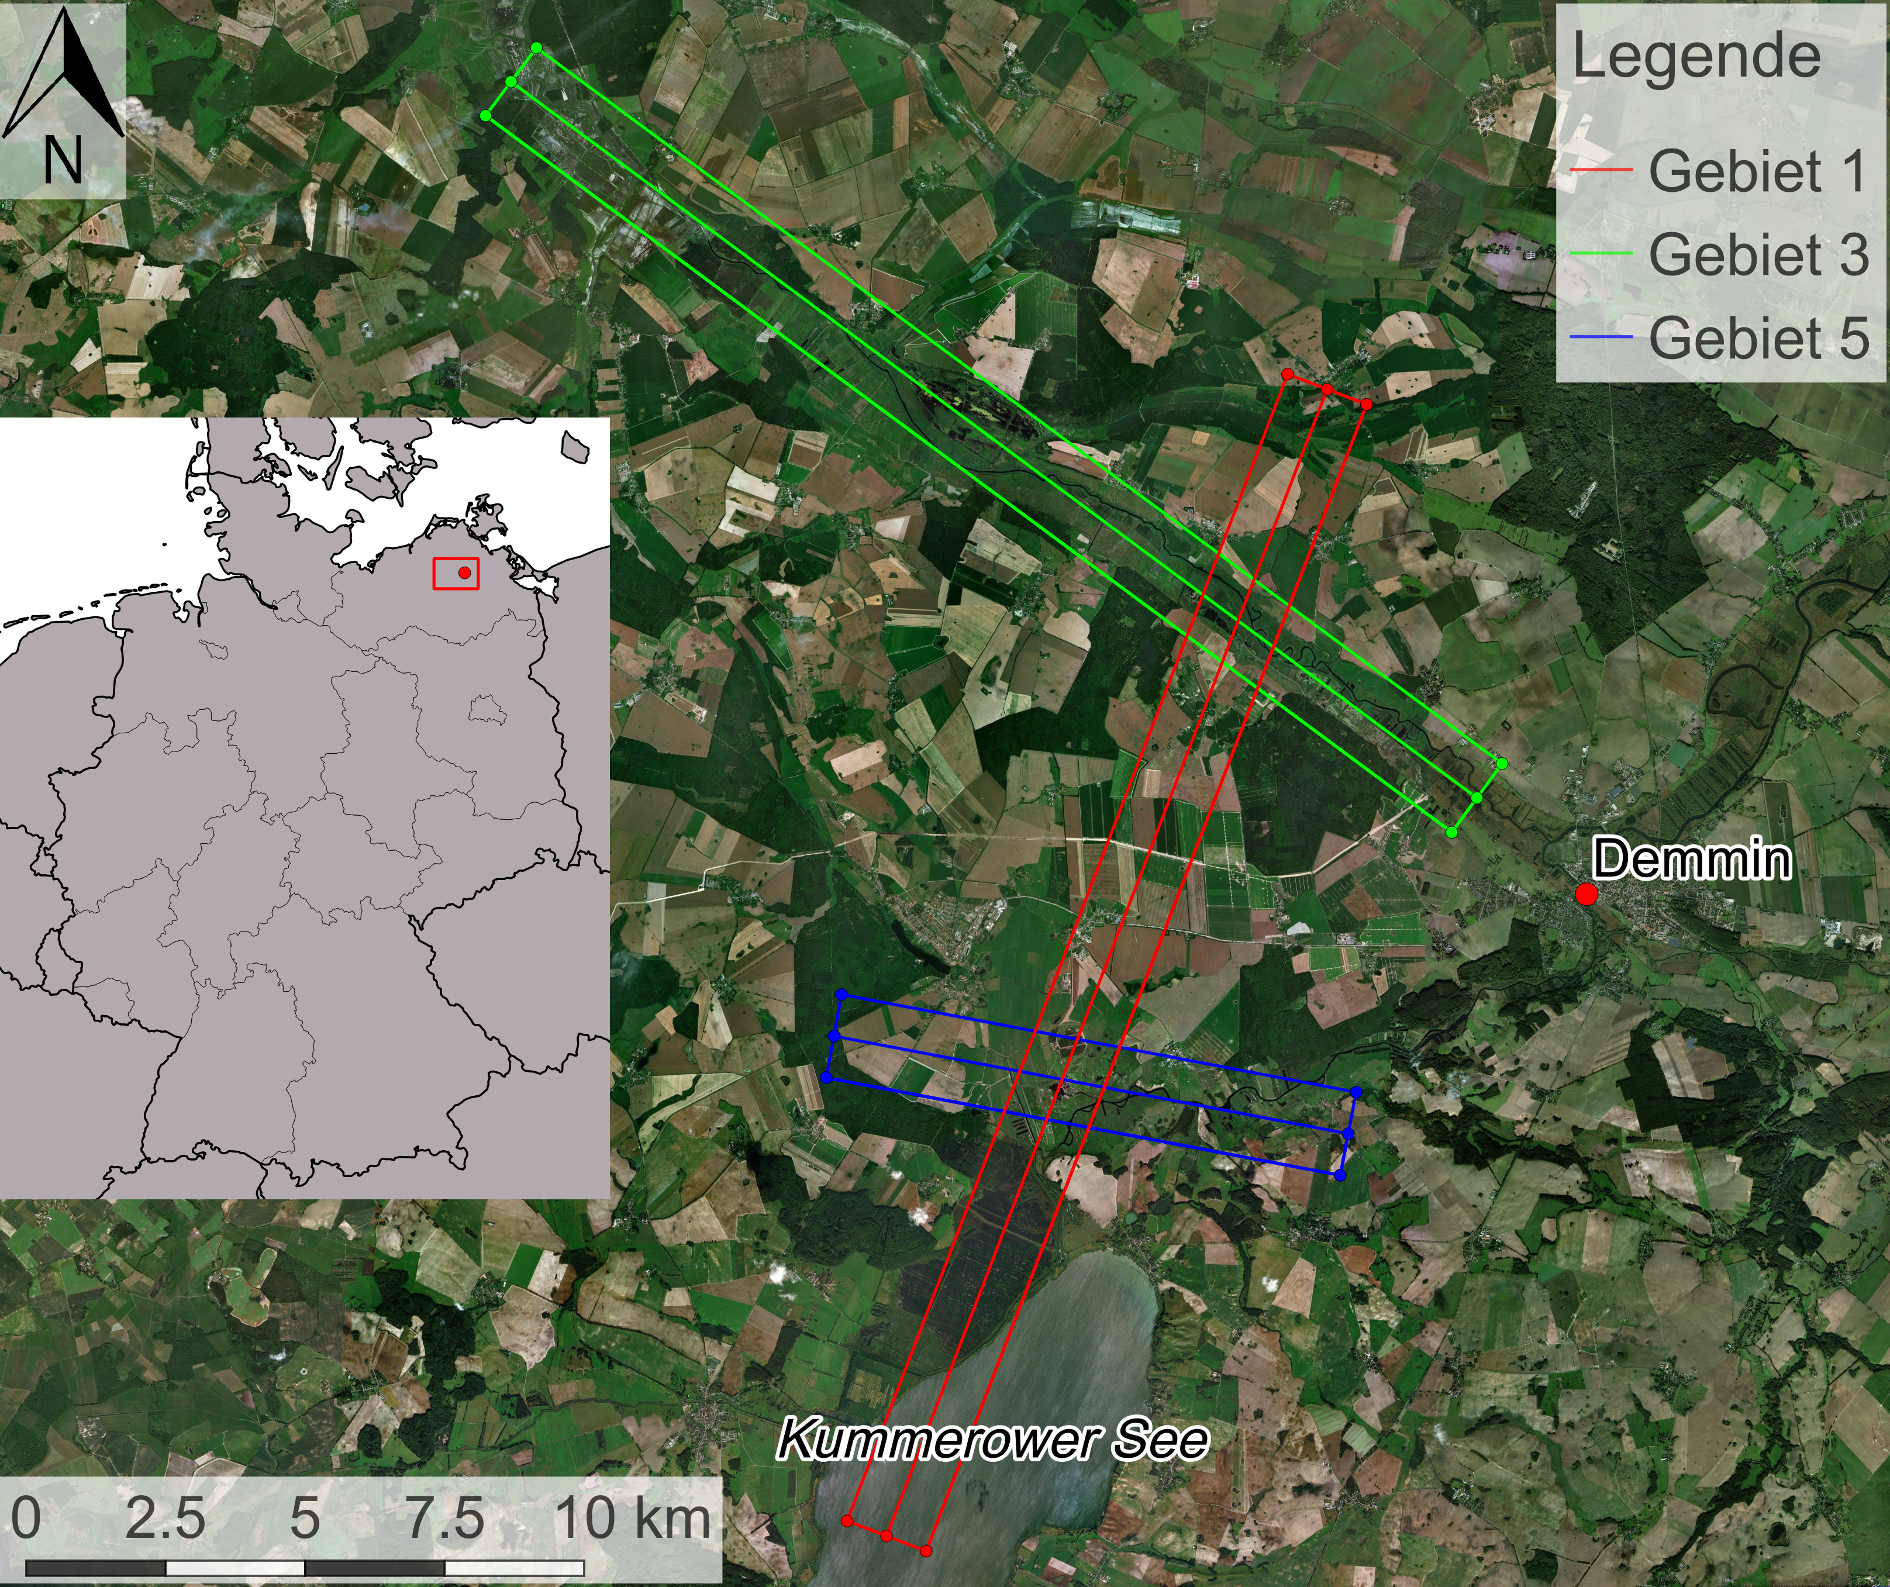
\includegraphics[width=\textwidth]{./docmedia/Gebietskarte.png}
				\caption{Bildflugtracks bei Demmin}
			\end{figure}
		\end{column}
	\end{columns}
\end{frame}

\section{Ergebnisse}

\subsection{Bestimmung der Konstanten}

\begin{frame}{Bestimmung der Konstanten}
	\begin{itemize}
		\item Langsam-Schnellflug, Korrektur des statischen Druckdefekts:
	\end{itemize}
	\begin{columns}
		\begin{column}{0.48\textwidth}
			\begin{figure}
				\includegraphics[width=\textwidth]{./docmedia/acc_dec_pattern.pdf}
				\caption{Fitting zur Bestimmung der Korrekturkonstanten}
			\end{figure}
		\end{column}
		\begin{column}{0.48\textwidth}
			\begin{figure}
				\includegraphics[width=\textwidth]{./docmedia/static_defect_reg.pdf}
				\caption{Verlauf von Staudruck und Flughöhe, 7. Juni 2018}
			\end{figure}
		\end{column}
	\end{columns}
\end{frame}

\begin{frame}{Bestimmung der Konstanten}
	\begin{itemize}
		\item Anströmwinkel
	\end{itemize}
	\begin{columns}
		\begin{column}{0.48\textwidth}
			\begin{figure}
				\includegraphics[width=\textwidth]{./docmedia/alpha_osz.pdf}
				\caption{Pitch-Oszillationsmanöver während eines Testfluges, 9. August 2017}
			\end{figure}
		\end{column}
		\begin{column}{0.48\textwidth}
			\begin{figure}
				\includegraphics[width=\textwidth]{./docmedia/beta_osz.pdf}
				\caption{Yaw-Oszillationsmanöver, gleicher Flug}
			\end{figure}
		\end{column}
	\end{columns}
\end{frame}

\subsection{Spektrale Leistungsdichte}

\begin{frame}{Spektrale Leistungsdichte}
	\begin{itemize}
		\item 1. und 2. Bildflug Demmin, 14. August 2018: 
	\end{itemize}
	\begin{figure}
		\includegraphics[width=.8\textwidth]{./docmedia/power_flights.pdf}
		\caption{Spektrale Leistungsdichten für die Windkomponenten, 14. August 2017}
	\end{figure}
\end{frame}

\section{Zusammenfassung}

\begin{frame}{Zusammenfassung und Ausblick}
	\begin{enumerate}
		\small
		\item Konzeption und Bau eines hochmobilen Turbulenz-/Gasflussmesssystems
		\item Implementierung Postprocessing
		\item Kalibrierung
		\begin{itemize}
			\item Isolierung von Fehlerquellen
		\end{itemize}
	\end{enumerate}
	\begin{block}{Ergebnisse}
		\begin{itemize}
			\item Kalibrierungsverfahren verbessert Windmessung ($\sigma_{u|v}\approx \pm 0.3 m\ s^{-1}$)
			\item größere Unsicherheiten in extremen Fluglagen
			\item Isolierung von Fehlerquellen nur eingeschränkt möglich
		\end{itemize}
	\end{block}
	\begin{block}{Verbesserungen}
		\begin{itemize}
			\item Einfluss Anströmwinkel auf statische Druckmessung
			\item schnelle Temperaturmessungen
			\item verifizierbare Vergleichsmessungen (EC-Turm Fly-by)
			\item Kopplung mit Gasanalyzer $\Rightarrow$ \alert{Gasflüsse}
		\end{itemize}
	\end{block}
\end{frame}

% All of the following is optional and typically not needed. 
\appendix
\section<presentation>*{\appendixname}
\subsection<presentation>*{For Further Reading}

\begin{frame}%[allowframebreaks]
  \frametitle<presentation>{Literatur (Auswahl)}
  \small
  \begin{thebibliography}{10}
    
  \beamertemplatebookbibitems
  % Start with overview books.

  \bibitem{anderson2010}
    J.~Anderson.
    \newblock {\em Fundamentals of Aerodynamics}.
    \newblock McGraw-Hill Education, 2010.
    
   \bibitem{lenshow1986}
     D.~H.~Lenschow.
     \newblock {Probing the atmospheric boundary layer}.
     \newblock {American Meteorological Society}, 1986.
  
  \beamertemplatearticlebibitems
  % Followed by interesting articles. Keep the list short. 

  \bibitem{drue2013}
    C.~Drüe und G.~Heinemann.
    \newblock {A review and practical guide to in-flight calibration for aircraft turbulence sensors}.
    \newblock {Journal of Atmospheric and Oceanic Technology}, 30(12): 2820–2837, 2013.
    
  \bibitem{axford1968}
    D.~N.~Axford.
    \newblock {On the accuracy of wind measurements using an inertial platform in an aircraft, and an example of a measurement of the vertical mesostructure of the atmosphere}.
    \newblock {Journal of Applied Meteorology}, 7:645–666, 1968.
    
  \bibitem{axford1968}
    W.~Bögel und R.~Baumann.
    \newblock {Test and calibration of the dlr falcon wind measuring system by maneuvers}.
    \newblock {Journal of Atmospheric and Oceanic Technology}, 8(1):5–18, 1991.
    
  \end{thebibliography}
\end{frame}

\begin{frame}
	\centering
	\Large Vielen Dank für die Aufmerksamkeit!
\end{frame}

\begin{frame}{Anhang}
	Synchronisierung
	\begin{figure}
		\includegraphics[width=.8\textwidth]{./docmedia/alp_plot_2.png}
		\caption{Zeitstempeldifferenzen eines Drucksensorlogs}
	\end{figure}
\end{frame}

\begin{frame}{Anhang}
	Synchronisierung
	\begin{figure}
		\includegraphics[width=.8\textwidth]{./docmedia/nova0_jitter.pdf}
		\caption{Zeitstempeldifferenz zwischen GPS-Zeit ($t_i$) und Systemzeitstempel ($t_{S,i}$) der IMU}
	\end{figure}
\end{frame}

\begin{frame}{Anhang}
	Bildfluggebiete
	\begin{figure}
		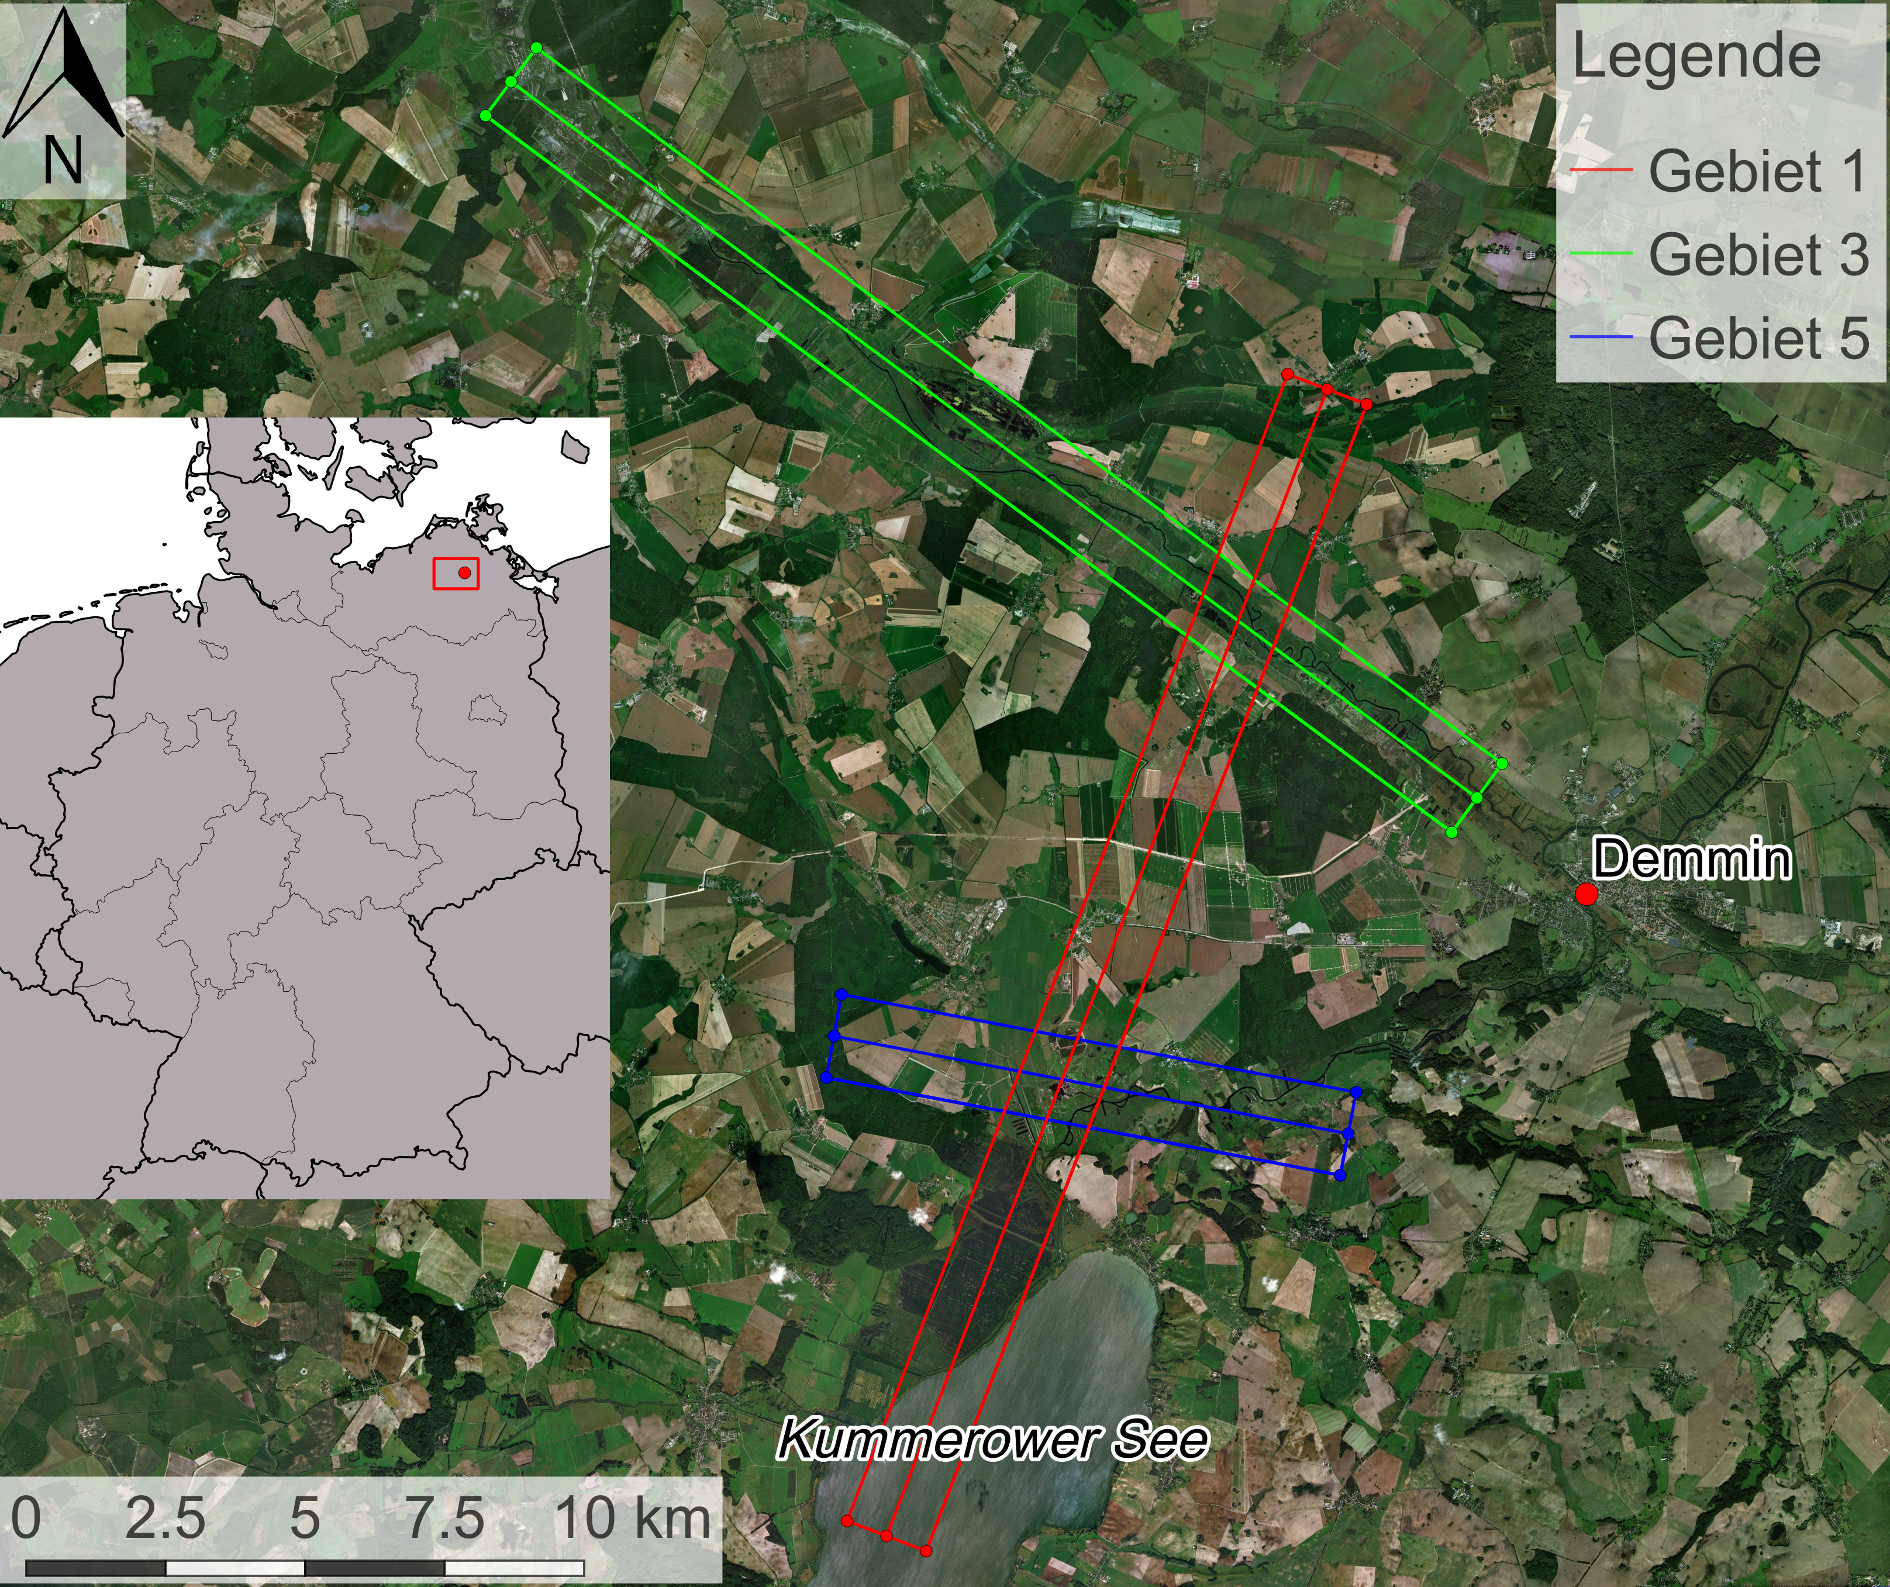
\includegraphics[width=.65\textwidth]{./docmedia/Gebietskarte.png}
		\caption{Bildfluggebiete von der Messkampagne bei Demmin (Mecklenburg-Vorpommern) am 14. und 15. August 2017}
	\end{figure}
\end{frame}

\begin{frame}{Anhang}
	\begin{figure}
		\includegraphics[width=.8\textwidth]{./docmedia/probe_inflight.jpg}
		\caption{Während eines Testfluges am 9. August 2017}
	\end{figure}
\end{frame}

\end{document}
